\documentclass{article} % Класс печатного документа

\usepackage[utf8]{inputenc} % Кодировка исходного текста - utf8
\usepackage[english,russian]{babel} % Поддержка языка - русского с английским
\usepackage{indentfirst} % Отступ в первом абзаце
\usepackage{amsmath} % Для символа точек в выборке
\usepackage{xfrac}
\usepackage{caption} % Для центрирования подписей к графике
\usepackage{float} % Для постановки графики точно где указано

\title{Лабораторная работа №2\\Ядерная оценка плотности распределения} % Заголовок документа
\author{Свичкарев А.\,В.\\группа 53601/4\\СПбПУ} % Автор документа
\date{\today} % Текущая дата

\begin{document} % Конец преамбулы, начало текста

\maketitle % Печатает заголовок, список авторов и дату

\section{Постановка задачи}
Дана выборка 100 элементов из стандартного нормального \mbox{распределения}:
\[x_1,x_2,\dotsc,x_{100}\sim\mathcal{N}(0,1)\]

Необходимо построить ядерные оценки плотности распределения, меняя значения параметра масштаба (bandwidth parameter) h:

\[\hat{f}_{n,h}(x) = \frac{1}{nh}K{\left(\frac{x-x_i}{h}\right)},\]

где $n$ -- размер выборки,\\
\indent $K$ -- гауссово ядро:

\[K(u) = \frac{1}{\sqrt{2\pi}}e^{\sfrac{-u^2}{2}}\]

Выборка из нормального распределения:
\\\newline

\input{../sample_N_0_1.txt}

\newpage
\section{Выполнение}
Используем рекомендацию Silverman'а по выбору h:

\[h_{Silverman} = \frac{S}{\sqrt[\leftroot{2}\uproot{2}5]{n}} \approx \frac{S}{2.51}\]

где \[S = \sqrt{\frac{1}{n}\sum_{i=1}^{n} (x_i-\bar{x})} = \frac{1}{10}\sqrt{\sum_{i=1}^{n}(x_i-\bar{x})}\]

Для текущей выборки $h_{Silverman} \approx 0.398$.

\begin{figure}[H]
    \captionsetup{justification=centering}
    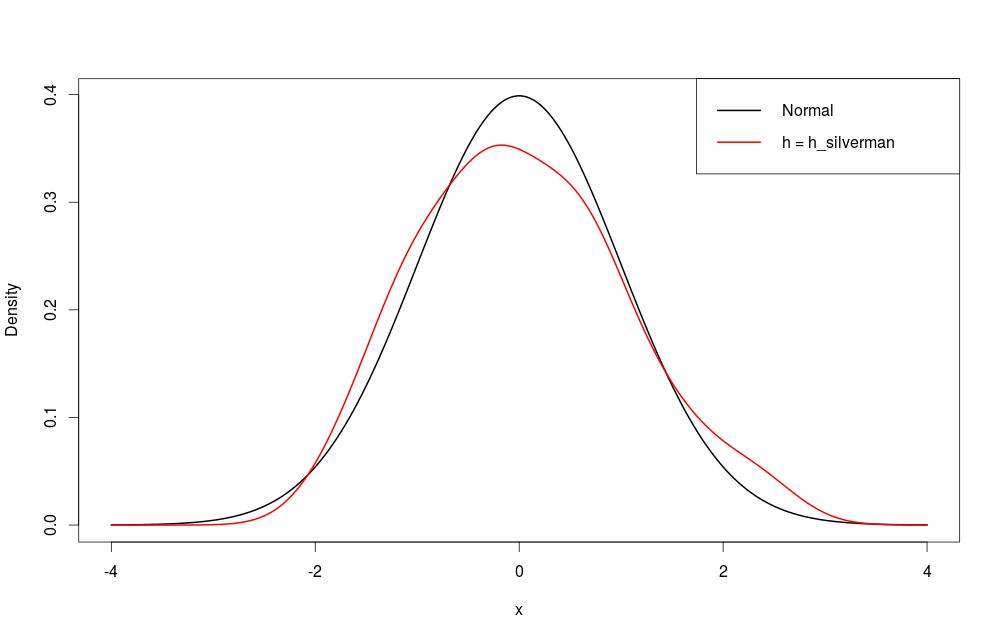
\includegraphics[width=\textwidth]{plot1}
    \caption{Сравнение плотности нормального распределения и ядерной оценки плотности с $h = h_{silverman}$.}
\end{figure}

\newpage
Попробуем взять другие h - в 2 раза больше и в два раза меньше, чем $h_{Silverman}$:

\begin{figure}[H]
    \captionsetup{justification=centering}
    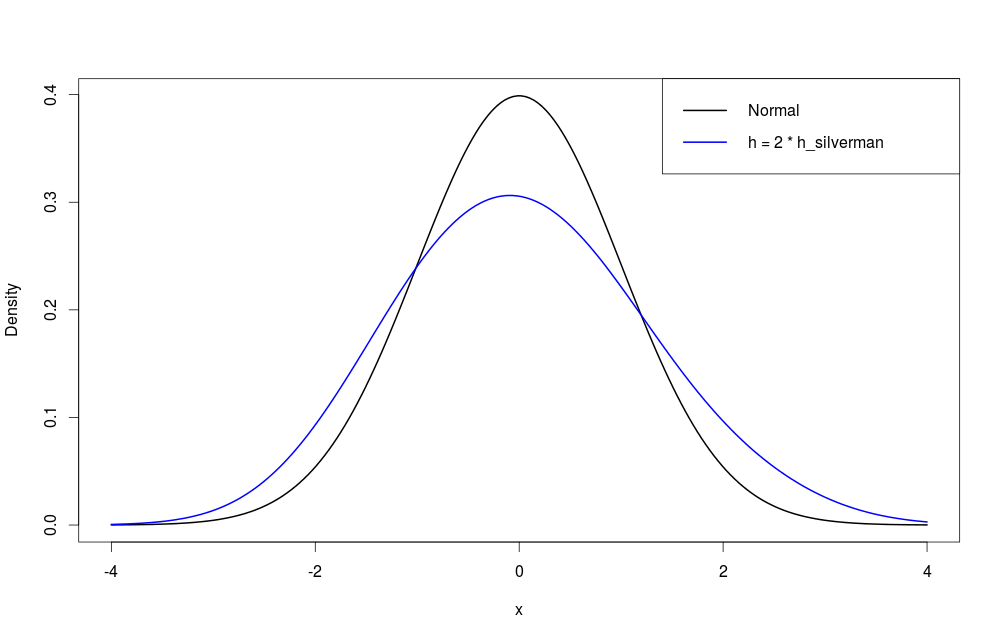
\includegraphics[width=0.9\textwidth]{plot2}
    \caption{Сравнение плотности нормального распределения и ядерной оценки плотности с $h = 2 h_{silverman}$.}
\end{figure}

\begin{figure}[H]
    \captionsetup{justification=centering}
    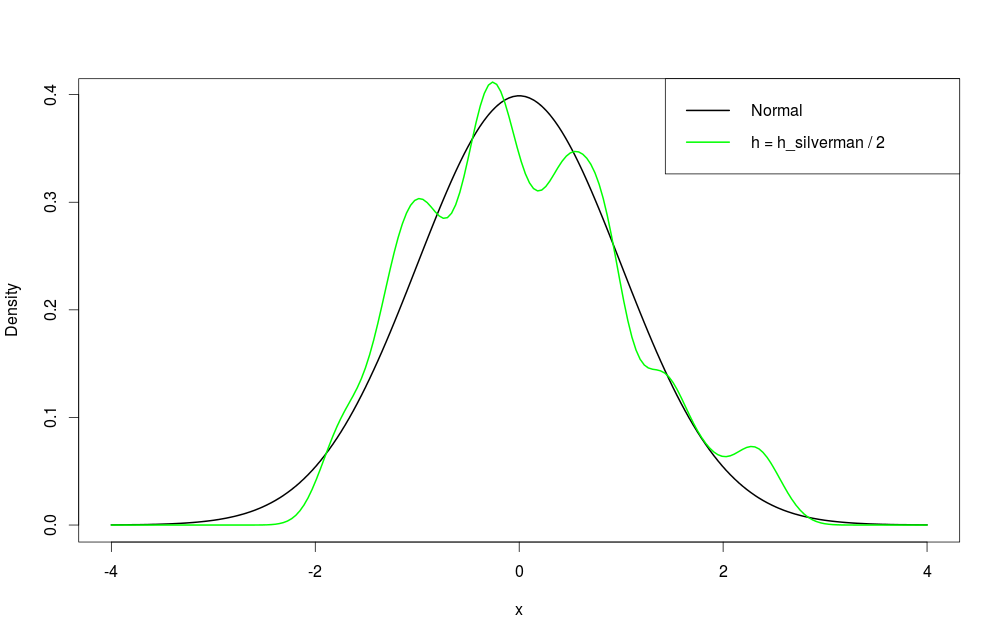
\includegraphics[width=0.9\textwidth]{plot3}
    \caption{Сравнение плотности нормального распределения и ядерной оценки плотности с $h = \frac{h_{silverman}}{2}$.}
\end{figure}

\section{Заключение}
При увеличении значения h оценка плотности распределения становится более гладкой и пологой.

При уменьшении h ядерная оценка плотности лучше покрывает график плотности распределения, однако появляется множество возмущений.

При ядерной оценке плотности вероятности нормального распределения имеет смысл брать значения bandwidth parameter близкие к значению $h_{Silverman}$.

\end{document} % Конец документа
